\documentclass{standalone}
\usepackage{pgfplots}
\pgfplotsset{compat=newest}
\begin{document}
Aligning at .......
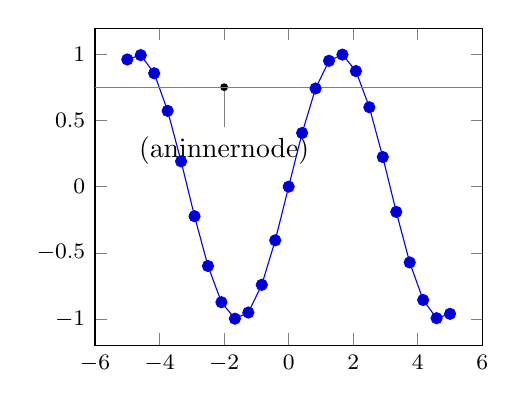
\begin{tikzpicture}[baseline]
\begin{axis}[small,anchor=aninnernode.center]
	\addplot {sin(deg(x))};
	\node
		[pin=-90:(aninnernode),fill=black,circle,scale=0.3] 
		(aninnernode) at (axis cs:-2,0.75) {};
	\draw[help lines] (axis cs:-6,0.75) -- (axis cs:6,0.75);
\end{axis}
\end{tikzpicture}
\end{document}
